\documentclass[a4paper,11pt,openright]{report}
\setlength{\parindent}{0pt} % set noindent for entire file

\usepackage[utf8]{inputenc}
\usepackage[a4paper,top=20mm,left=10mm,right=15mm]{geometry}
\usepackage{xcolor,graphicx}
\usepackage{amsmath}
\usepackage{setspace}
\usepackage{sectsty}
\usepackage{etoolbox}
\usepackage{enumitem}
\usepackage{listings}
\usepackage{times}

\graphicspath{ {/home/saran/Analytics/May_05/} }

\lstdefinestyle{mystyle}{
	backgroundcolor=\color{white},
	basicstyle=\ttfamily\footnotesize,
	breakatwhitespace=false,
	breaklines=true,
	captionpos=b,
	keepspaces=true,
	showspaces=false,
	showstringspaces=false,
	showtabs=false,
	tabsize=4
}

\lstset{style=mystyle}

\begin{document}
\singlespacing
\pagestyle{plain}

\begin{center}
\textbf{Assignment T-test} \\
Date: 05/05/2020 \hspace{2mm} Name: D.Saravanan
\end{center}

\vspace{10px}

TTest test the null hypothesis $H_{0}$ against the alternative hypothesis $H_{1}$. \\

For univariate samples, TTest performs a Student $t$ test. The test statistic is assumed to
follow a StudentTDistribution [df]. \\ 

The degrees of freedom df, used to specify the distribution of the test statistic, depend on
the sample size, number of samples, and in the case of two univariate samples, the results 
of a test for equal variances. \\ 

For the TTest, a cutoff $\alpha$ is chosen such that $H_{0}$ is rejected only if $p < \alpha
$. The value of $\alpha$ used for the "TestConclusion" and "ShortTestConclusion" properties 
is controlled by the SignificanceLevel option. This value $\alpha$ is also used in diagnostic
tests of assumptions, including tests for normality, equal variance, and symmetry. By 
default, $\alpha$ is set to $0.05$. 

\begin{enumerate}

\item[1.] Two sets of ten students selected at random from a college were taken. One set was
given memory test as they were and the other was given the memory test after two weeks of
training and the scores are given below. \\
\begin{tabular}{lrrrrrrrrrr}
Set A: & 10 & 8 & 7 & 9 & 8 & 10 & 9 & 6 & 7 & 8 \\ 
Set B: & 12 & 8 & 8 & 10 & 8 & 11 & 9 & 8 & 9 & 9 \\
\end{tabular} \\
Do you think there is a significant effect due to training? \\

\textbf{Solution:}

\textbf{Set A:} \\ 
\hspace*{10mm} Mean:
\begin{equation*}
\bar x_{1} = \frac{\sum\limits_{i=1}^{n1} x_{1i}}{n1}
    	= \frac{10 + 8 + 7 + 9 + 8 + 10 + 9 + 6 + 7 + 8}{10}
    	= 8.2
\end{equation*}

\hspace*{10mm} Variance:
\begin{equation*}
s_{1}^{2} = \frac{\sum\limits_{i=1}^{n1} (x_{1i} - \bar {x_{1}})^{2}}{n1 - 1}
		= \frac{\sum\limits_{i=1}^{10} (x_{1i} - 8.2)^{2}}{10 -1} = 1.73333
\end{equation*}

\hspace*{10mm} Standard Deviation:
\begin{equation*}
s_{1} = \sqrt{\frac{\sum\limits_{i=1}^{n1} (x_{1i} - \bar {x_{1}})^{2}}{n1 - 1}}
	= \sqrt{\frac{\sum\limits_{i=1}^{10} (x_{1i} - 8.2)^{2}}{10 -1}}
	= \sqrt{1.73333} = 1.31656
\end{equation*}

\textbf{Set B:} \\
\hspace*{10mm} Mean:
\begin{equation*}
\bar x_{2} = \frac{\sum\limits_{i=1}^{n2} x_{2i}}{n2}
	= \frac{12 + 8 + 8 + 10 + 8 + 11 + 9 + 8 + 9 + 9}{10}
	= 9.2
\end{equation*}

\hspace*{10mm} Variance:
\begin{equation*}
s_{2}^{2} = \frac{\sum\limits_{i=1}^{n2} (x_{2i} - \bar {x_{2}})^{2}}{n2 - 1}
= \frac{\sum\limits_{i=1}^{10} (x_{2i} - 9.2)^{2}}{10 -1} = 1.95556
\end{equation*}

\hspace*{10mm} Standard Deviation:
\begin{equation*}
s_{2} = \sqrt{\frac{\sum\limits_{i=1}^{n2} (x_{2i} - \bar x_{2})^{2}}{n2 - 1}}
= \sqrt{\frac{\sum\limits_{i=1}^{10} (x_{2i} - 9.2)^{2}}{10 -1}}
= \sqrt{1.95556} = 1.39841
\end{equation*} \\

Calculation of $s1/s2$:
\begin{equation*}
\frac{s_{1}}{s_{2}} = \frac{1.31656}{1.39841} = 0.94147
\end{equation*}

Test statistic: 
\begin{equation*}
T = \frac{\bar x_{1} - \bar x_{2}}{\sqrt{s_{1}^{2}/n1 + s_{2}^{2}/n2}}
\end{equation*}

where $n1$ and $n2$ are the sample sizes, $\bar x_{1}$ and $\bar x_{2}$ are the sample
means, and $s_{1}^{2}$ and $s_{2}^{2}$ are the sample variances. 

If equal variances are assumed $(0.5 < s1/s2 < 2)$, then the formula reduces to:
\begin{equation*}
T = \frac{\bar x_{1} - \bar x_{2}}{s_{p} \sqrt{1/n1 + 1/n2}}
\end{equation*}

where
\begin{equation*}
s_{p}^{2} = \frac{(n1-1)s_{1}^{2} + (n2-1)s_{2}^{2}}{n1+n2-2}
\end{equation*}

Calculation of $s_{p}$:
\begin{equation*}
s_{p} = \sqrt{\frac{(10-1) \times 1.31656^{2} + (10-1) \times 1.39841^{2}}{10+10-2}} 
      = 1.35810
\end{equation*}

Calculation of T statistic:
\begin{equation*}
T = \frac{8.2 - 9.2}{1.35810 \times \sqrt{1/10 + 1/10}} = -1.64646
\end{equation*}

Calculation of Standard Error:
\begin{equation*}
S.E = s_{p} \sqrt{1/n1 + 1/n2} = 1.35810 \times \sqrt{1/10 + 1/10} = 0.60736
\end{equation*}

\vspace{2cm}

Program:
\lstinputlisting[language=Python]{tscript3.py}

\vspace{2cm}

Output:
\lstinputlisting{toutput31.txt}

%figure_1
\begin{figure}[ht!]
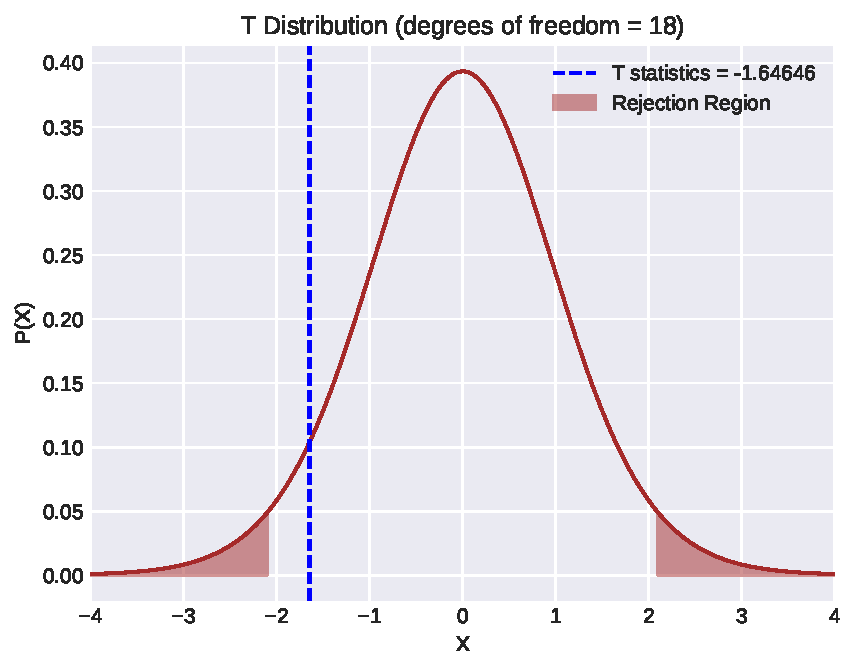
\includegraphics[width=16cm,height=8cm,keepaspectratio]{tscript3.pdf}
\centering
\end{figure}

\vspace{2cm}

Program: T-test with in-built scipy.stats.ttest
\lstinputlisting[language=Python]{ttest2.py}

\vspace{2cm}

Output:
\lstinputlisting{toutput32.txt}

%figure_2
\begin{figure}[ht!]
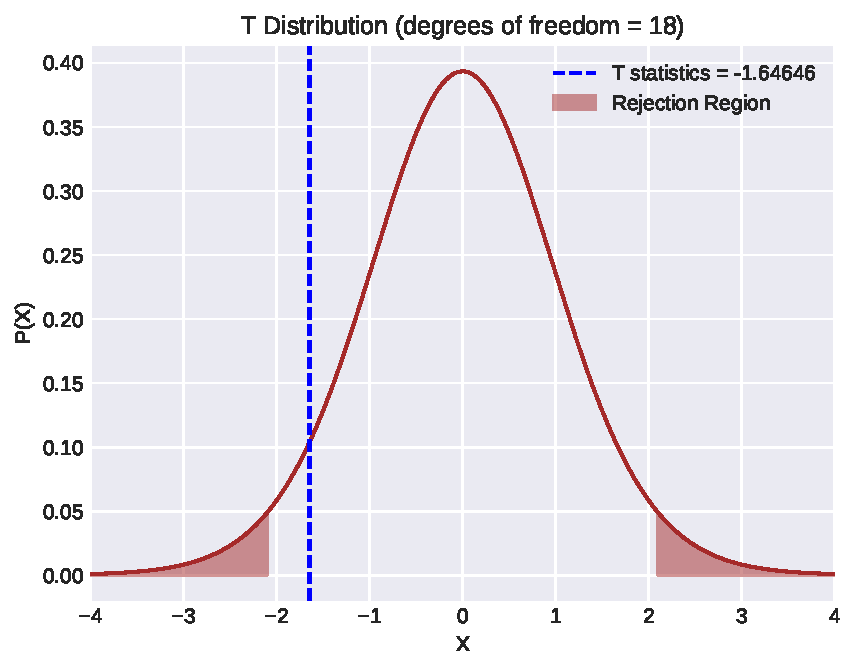
\includegraphics[width=16cm,height=8cm,keepaspectratio]{ttest2.pdf}
\centering
\end{figure}

\pagebreak

\item[2.] A group of 5 patients treated with medicine A weighs 42, 29, 48, 60 and 41 kg.
A second group of 7 patients from the same hospital treated with medicine B weighs 38, 42,
56, 64, 68, 69 and 62 kg. Do you agree with the claim that medicine B increases weight
significantly. \\

Null hypothesis: $H_{0}: \mu 1 = \mu 2$ \\
Alternative hypothesis: $H_{1}: \mu 1 \neq \mu 2$ \\

Medicine A: \\
\hspace*{10mm} Mean:
\begin{equation*}
\bar x_{1} = \frac{\sum\limits_{i=1}^{n1} x_{1i}}{n1}
		= \frac{42 + 29 + 48 + 60 + 41}{5} = 44.0
\end{equation*}

\hspace*{10mm} Variance:
\begin{equation*}
s_{1}^{2} = \frac{\sum\limits_{i=1}^{n1} (x_{1i} - \bar {x_{1}})^{2}}{n1 - 1}
	= \frac{\sum\limits_{i=1}^{5} (x_{1i} - 44.0)^{2}}{5 - 1} = 127.5
\end{equation*}

\hspace*{10mm} Standard Deviation:
\begin{equation*}
s_{1} = \sqrt{\frac{\sum\limits_{i=1}^{n1} (x_{1i} - \bar {x_{1}})^{2}}{n1 - 1}}
	= \sqrt{\frac{\sum\limits_{i=1}^{5} (x_{1i} - 44.0)^{2}}{5 -1}}
	= \sqrt{127.5} = 11.29159
\end{equation*}

Medicine B: \\
\hspace*{10mm} Mean:
\begin{equation*}
\bar x_{1} = \frac{\sum\limits_{i=1}^{n1} x_{1i}}{n1}
		= \frac{38 + 42 + 56 + 64 + 68 + 69 + 62}{7} = 57.0
\end{equation*}

\hspace*{10mm} Variance:
\begin{equation*}
s_{1}^{2} = \frac{\sum\limits_{i=1}^{n1} (x_{1i} - \bar {x_{1}})^{2}}{n1 - 1}
	= \frac{\sum\limits_{i=1}^{7} (x_{1i} - 57.0)^{2}}{7 - 1} = 154.3
\end{equation*}

\hspace*{10mm} Standard Deviation:
\begin{equation*}
s_{1} = \sqrt{\frac{\sum\limits_{i=1}^{n1} (x_{1i} - \bar {x_{1}})^{2}}{n1 - 1}}
	= \sqrt{\frac{\sum\limits_{i=1}^{7} (x_{1i} - 57.0)^{2}}{7 -1}}
	= \sqrt{154.3} = 12.42310
\end{equation*}

Calculation of $s1/s2$:
\begin{equation*}
\frac{s_{1}}{s_{2}} = \frac{11.29159}{12.42310} = 0.90892
\end{equation*}

Test statistic:
\begin{equation*}
T = \frac{\bar x_{1} - \bar x_{2}}{\sqrt{s_{1}^{2}/n1 + s_{2}^{2}/n2}}
\end{equation*}

If equal variances are assumed $(0.5 < s1/s2 < 2)$, then the formula reduces to:
\begin{equation*}
T = \frac{\bar x_{1} - \bar x_{2}}{s_{p} \sqrt{1/n1 + 1/n2}}
\end{equation*}

where
\begin{equation*}
s_{p}^{2} = \frac{(n1-1)s_{1}^{2} + (n2-1)s_{2}^{2}}{n1+n2-2}
\end{equation*}

Calculation of $s_{p}$:
\begin{equation*}
s_{p} = \sqrt{\frac{(5-1) \times 11.29159^{2} + (7-1) \times 12.42310^{2}}{5+7-2}} 
      = 11.98332
\end{equation*}

Calculation of T statistic:
\begin{equation*}
T = \frac{44.0 - 57.0}{11.98332 \times \sqrt{1/5 + 1/7}} = -1.85272
\end{equation*}

Calculation of Standard Error:
\begin{equation*}
S.E = s_{p} \sqrt{1/n1 + 1/n2} = 11.98332 \times \sqrt{1/5 + 1/7} = 7.01671
\end{equation*}

Program:
\lstinputlisting[language=Python]{tscript3.py}
Output:
\lstinputlisting{toutput41.txt}

%figure_3
\begin{figure}[ht!]
\includegraphics[width=16cm,height=8cm,keepaspectratio]{tscript41.pdf}
\centering
\end{figure}

Program: T-test with in-built scipy.stats.ttest
\lstinputlisting[language=Python]{ttest2.py}
Output:
\lstinputlisting{toutput42.txt}

%figure_4
\begin{figure}[ht!]
\includegraphics[width=16cm,height=8cm,keepaspectratio]{tscript42.pdf}
\centering
\end{figure}

\item[3.] Samples of two types of electric bulbs were tested for length of life and the
following data were obtained \\
\begin{tabular}{lrr}
		& Type I & Type II \\
No. of Samples: & 8 & 7 \\
Mean (hours):   & 1134 & 1024 \\
SD (hours):     & 35 & 40 \\
\end{tabular} \\
Test at 5 percent level, whether the difference in sample mean is significant. \\

Null hypothesis: $H_{0}: \mu 1 = \mu 2$ \\
Alternative hypothesis: $H_{1}: \mu 1 \neq \mu 2$ \\

Type I: \\
\hspace*{10mm} Mean = 1134 \\
\hspace*{10mm} Variance = 1225 \\
\hspace*{10mm} Standard Deviation = 35

Type II: \\
\hspace*{10mm} Mean = 1024 \\
\hspace*{10mm} Variance = 1600 \\
\hspace*{10mm} Standard Deviation = 40

Calculation of $s1/s2$:
\begin{equation*}
\frac{s_{1}}{s_{2}} = \frac{35}{40} = 0.875
\end{equation*}

Test statistic: 
\begin{equation*}
T = \frac{\bar x_{1} - \bar x_{2}}{\sqrt{s_{1}^{2}/n1 + s_{2}^{2}/n2}}
\end{equation*}

where $n1$ and $n2$ are the sample sizes, $\bar x_{1}$ and $\bar x_{2}$ are the sample
means, and $s_{1}^{2}$ and $s_{2}^{2}$ are the sample variances. 

If equal variances are assumed $(0.5 < s1/s2 < 2)$, then the formula reduces to:
\begin{equation*}
T = \frac{\bar x_{1} - \bar x_{2}}{s_{p} \sqrt{1/n1 + 1/n2}}
\end{equation*}

where
\begin{equation*}
s_{p}^{2} = \frac{(n1-1)s_{1}^{2} + (n2-1)s_{2}^{2}}{n1+n2-2}
\end{equation*}

Calculation of $s_{p}$:
\begin{equation*}
s_{p} = \sqrt{\frac{(8-1) \times 35^{2} + (7-1) \times 40^{2}}{8+7-2}} 
      = 37.39087
\end{equation*}

Calculation of T statistic:
\begin{equation*}
T = \frac{1134 - 1024}{37.39087 \times \sqrt{1/8 + 1/7}} = 5.68428
\end{equation*}

Calculation of Standard Error:
\begin{equation*}
S.E = s_{p} \sqrt{1/n1 + 1/n2} = 37.39087 \times \sqrt{1/8 + 1/7} = 19.35161
\end{equation*}

\end{enumerate}
\end{document}
